\documentclass[12pt,a4paper]{book}
\usepackage[minitoc]{teach}
\usepackage[utf8]{inputenc}
\usepackage[french]{babel}
\usepackage[T1]{fontenc}
\usepackage{amsmath}
\usepackage{amsfonts}
\usepackage{amssymb}
\usepackage{graphicx}
\renewcommand{\headrulewidth}{0pt}
\renewcommand{\footrulewidth}{0pt}
\fancyfoot[C]{\thepage}


\author{YAWO Kossi Atsu}
\newcommand{\prof}{YAWO Kossi Atsu}
\newcommand{\matiere}{\\PHYSIQUE- CHIMIE- TECHNOLOGIE}
\newcommand{\classe}{6$^{ème}$}
\title{Mes devoirs de \matiere}
\begin{document}
\begin{td}{\matiere}{\classe}{12 octobre 2019}{\prof}
\begin{exo}
Yapo a noté les température suivantes: $32\degres C$ dans la pièce; $8 \degres C$ dans le réfrigérateur et $-5\degres C$ dans le compartiment à glace. Il place un morceau de glace dans un verre. Que trouvera-t-il dans le verre, au bout d'une heure par exemple 'il l'abandonne:
\begin{enumerate}
\item dans la pièce?
\item dans le réfrigérateur?
\item dans le compartiment à glace?
\end{enumerate} 
\end{exo}
\vspace{0.5cm}

\begin{exo}
\begin{multicols}{2}
Un groupe d'élèves A a relevé les températures au cours du chauffage d'une substance qui reste liquide durant l'expérience. Un autre groupe d'élèves B a relevé les températures au cours du chauffage d'un corps qui subit une fusion. Analyse les graphiques suivants et pour chacun le groupe qui l'a tracé en justifiant ton choix.
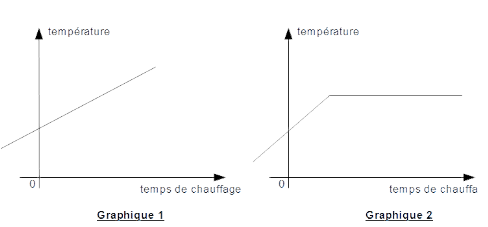
\includegraphics[scale=0.8]{images/img1_19102019.png}
\end{multicols}
\end{exo}
\vspace{0.5cm}

\begin{exo}
On a relevé des températures de refroidissement de l'eau toutes les minutes.
\begin{multicols}{2}
\begin{enumerate}
\item Quelle est la température de l'eau au début de cette expérience? 
\item Pendant combien de minutes n'a-t-on eu que de l'eau liquide?
\item Combien de temps a duré le changement d'état de l'eau?
\end{enumerate}
\vspace{2cm}
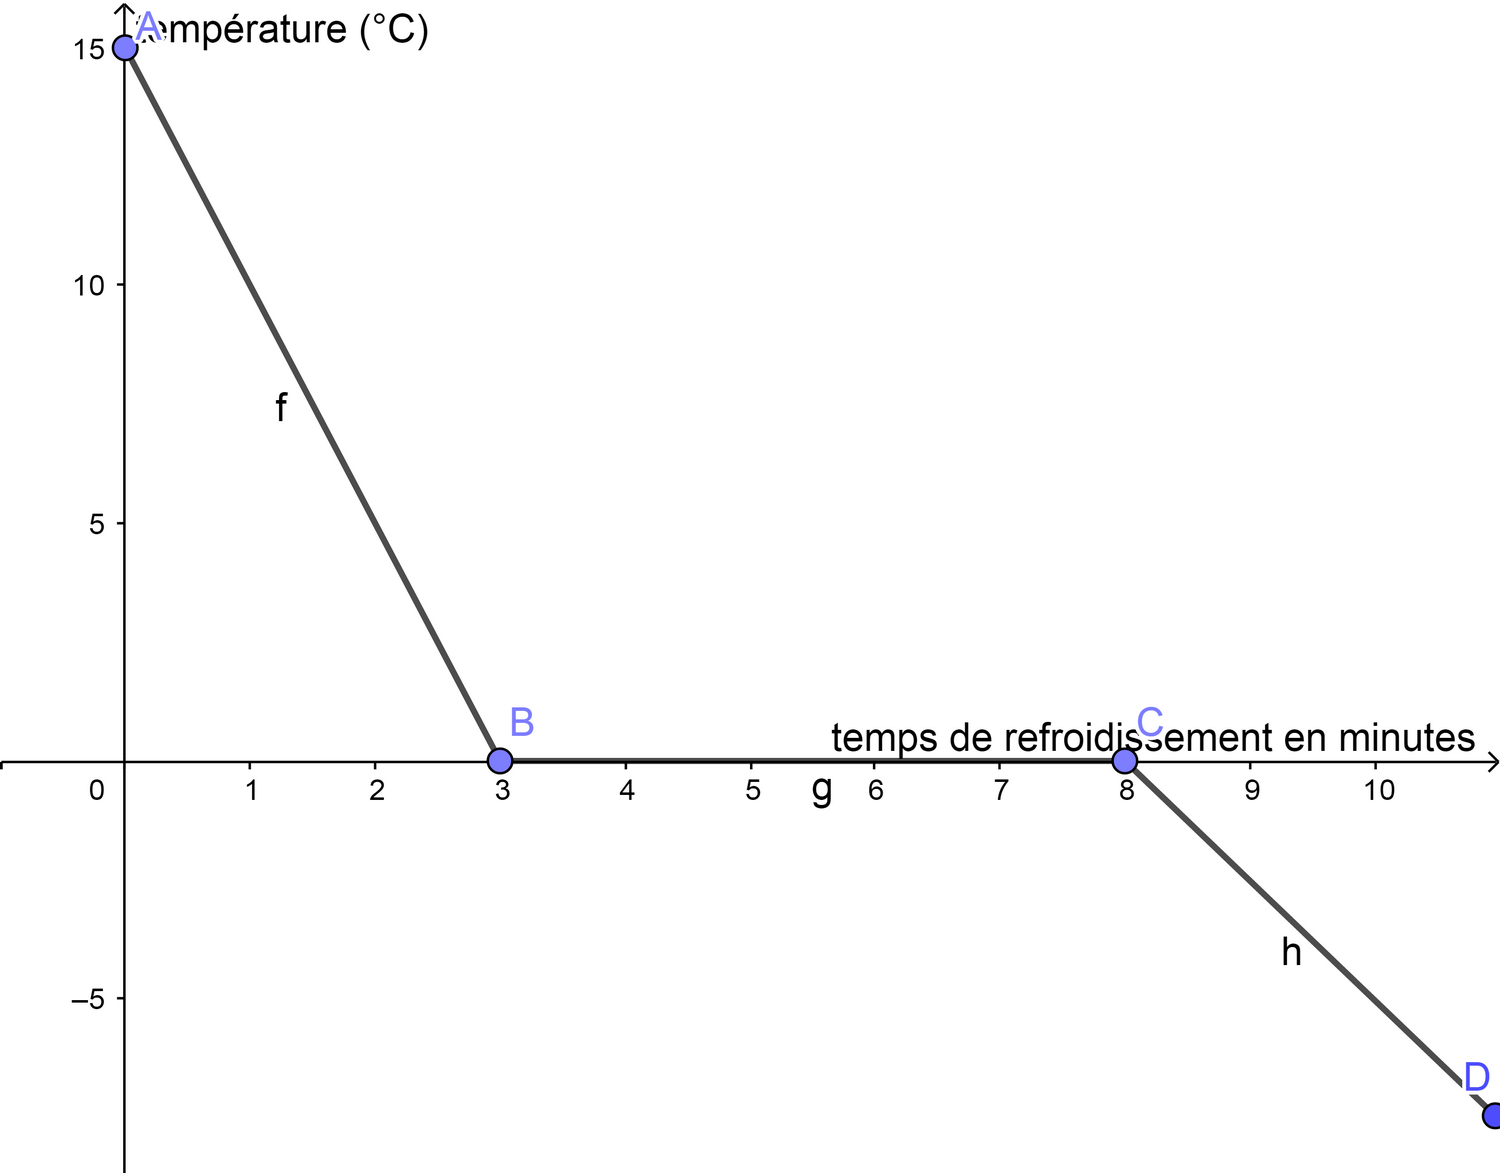
\includegraphics[scale=1]{images/refroidissement_cor.png}
\end{multicols}
\end{exo}
\vspace{0.5cm}

\begin{exo}
\begin{enumerate}
\item Qu'est-ce que la matière?
\item Quels sont les états de la matière?
\item Donne pour chaque état de la matière deux exemples d'objet.
\item Reproduis puis complète le tableau suivant en mettant une croix (X) dans la case qui convient:
\begin{tabular}{|p{4cm}|p{4cm}|p{4cm}|p{4cm}|}
\hline
• & Solides & Liquides & Gaz \\  
\hline 
Ont une forme propre &  &  &  \\ 
\hline 
Sont saisissable &  &  &  \\ 
\hline 
Ont un volume &  &  &  \\ 
\hline 
\end{tabular} 
\end{enumerate}
\end{exo}
\end{td}

\begin{td}{\matiere}{\classe}{09 novembre 2019}{\prof}
\begin{exo}
Choisis la bonne réponse:
\begin{multicols}{2}
\begin{enumerate}
\item Les liquides deviennent solides si on les
\begin{enumerate}
\item refroidir convenablement.
\item chauffe convenablement.
\end{enumerate}

\item Lorsque les liquides devienne solides:
\begin{enumerate}
\item il y a variation de volume.
\item il n'y a pas variation de volume.
\end{enumerate}

\item Lorsque les liquides deviennent solides
\begin{enumerate}
\item il y a variation de masse.
\item il n'y a pas variation de masse.
\end{enumerate}

\item La vapeur d'eau est:
\begin{enumerate}
\item visible.
\item invisible.
\end{enumerate}
\end{enumerate}

\end{multicols}
\end{exo}

\vspace{0.5cm}
\begin{exo}
\begin{enumerate}
\item Classe par ordre de volume croissant:\\
$90cl$ \qquad ;\qquad $750 cm^3$ \qquad ;\qquad $25dl$ \qquad ;\qquad $150ml$ \qquad ;\qquad $10cm^3$ 
\item L'épaisseur d'une rame de 500 feuilles de papier de format $29,7 cm\times 21,0cm$ est égale à $7,5cm$. Calcule le volume d'une seule feuille de papier.
\item La contenance d'une cuillère à café ou d'une cuillère à soupe est utilisée, parfois, pour exprimer une quantité de liquide (sirop, médicament). Comment peut- on déterminer leur contenance avec une précision convenable?
\item Un morceau de sucre a les dimension suivantes: $27,5 mm$ \qquad ; \qquad $18 mm$ \qquad ; \qquad et $11,3mm$. 
\begin{enumerate}
\item Calcule son volume en $cm^3$. Pourrais-tu mesurer
\item Pourrais-tu mesurer ce volume à l'aide d'une éprouvette graduée? Explique.
\end{enumerate} 
\end{enumerate}
\end{exo}

\vspace{0.5cm}
\begin{exo}
Marie et Jeanne font une expérience. Elles ont chacune un bocal rempli de glace dans lequel elle ont mis un thermomètre. Marie met son bocal la table et Jeanne met le sien dans une casserole d'eau tiède. Elles lisent toutes les deux leur thermomètre quand la glace est en train de fondre.
\begin{enumerate}
\item Est-ce que Marie lit une température:
\begin{itemize}
\item plus élevée que celle lue par Jeanne?
\item égale à celle lue par Jeanne?
\item Plus basse que celle lui par Jeanne?
\end{itemize}
\item Indiquez la ou les températures lues?
\end{enumerate}
\end{exo}

\vspace{0.5cm}
\begin{exo}
\begin{enumerate}
\item Définis les termes suivant: la technologie, un objet naturel, un objet technique; une famille d'objet.
\item Donne trois exemples d'objets naturels; trois exemples d'objets techniques et un exemple de famille d'objets.
\item Un maçon veut fabriquer des briques:
\begin{enumerate}
\item cite deux objets naturels dont il a besoin.
\item cite deux objets technique dont il a besoin.
\end{enumerate}
\item Quelle est la différence entre une pierre et un caillou?
\end{enumerate}
\end{exo}
\end{td}



\begin{devoir}{DEVOIR SURVEILLE DU PREMIER TRIMESTRE}{\matiere}{\classe}{1}{1H 30}{13 novembre 2019}{\prof}
\begin{exo}[8]
\begin{multicols}{2}
Martine et Augustine font une expérience. Elles ont chacune un bocal rempli de glace dans lequel elle ont mis un thermomètre. Martine met son bocal la table et Augustine met le sien dans une casserole d'eau tiède. Elles lisent toutes les deux leur thermomètre quand la glace est en train de fondre.

\vspace{0.5cm}

\underline{\textbf{Consignes}}\\
Réponds aux questions suivantes et explique.
\begin{enumerate}
\item Est-ce que Martine lit une température:
\begin{itemize}
\item plus élevée que celle lue par Augustine?
\item égale à celle lue par Augustine?
\item Plus basse que celle lui par Augustine?
\end{itemize}
\item Indiquez la ou les températures lues?
\end{enumerate}

\end{multicols}
\begin{tabular}{|c|c|c|c|c|}
\hline 
Critère & Pertinence & Correction & Cohérence & Perfectionnement \\ 
\hline
Barème & 2pts & 2pts & 3pts & 1pt \\ 
\hline 
\end{tabular}

\competence{•}{8}
\end{exo}

\begin{exo}[7]
\begin{multicols}{2}
\begin{enumerate}
\item Classe par ordre de volume croissant:\\
$90cl$ \qquad ;\qquad $750 cm^3$ \qquad ;\qquad $25dl$ \qquad ;\qquad $150ml$ \qquad ;\qquad $10cm^3$ 
\competence{•}{2}
\item L'épaisseur d'une rame de 500 feuilles de papier de format $29,7 cm\times 21,0cm$ est égale à $7,5cm$. Calcule le volume d'une seule feuille de papier.
\competence{•}{2}
\item Détermine le volume du solide plongé dans le liquide.\\
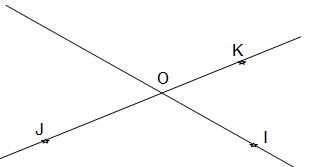
\includegraphics[scale=0.9]{images/dev120192020img1.png}
\item \underline{\textbf{Réponds par vrai ou faux aux affirmations suivantes}} 
\begin{enumerate}
\item Le passage d'un corps de l'état solide à l'état liquide s'appelle la solidification.
\item 0° C est la plus grande température que peut atteindre la glace.
\item L'eau bout à 90° C.
\item Les liquides ont un volume invariable.
\end{enumerate}

\competence{•}{1}
\end{enumerate}
\end{multicols}
\end{exo}

\vspace{0.5cm}
\begin{exo}[5]
\begin{enumerate}
\item Définis les termes suivant: un objet naturel, un objet technique; une famille d'objet.
\item Donne trois exemples d'objets naturels; trois exemples d'objets techniques et un exemple de famille d'objets.
\item Un maçon veut fabriquer des briques:
\begin{enumerate}
\item cite deux objets naturels dont il a besoin.
\item cite deux objets technique dont il a besoin.
\end{enumerate}
\end{enumerate}
\competence{•}{5}
\end{exo}

\tableofcompetences
\end{devoir}

\newpage

\begin{td}{\matiere}{\classe}{07 décembre 2019}{\prof}
\begin{exo}
Koffi a mesuré la masse d'une bougie et trouve $m=42,8g$. Il allume cette bougie qui s'éteint quelques instants après. Une deuxième pesée lui donne une nouvelle masse $m'=41,6g$.
\begin{enumerate}
\item \begin{enumerate}
\item Pourquoi la masse de la bougie a-t-elle diminuée?
\item De combien a-t-elle diminuée?
\end{enumerate}
\item La bougie allumée a été coiffée par un flacon contenant $1,5l$ d'air. Calcule la masse de bougie qui brûle dans $1l$ d'air.
\item Après la combustion, on verse un liquide limpide et incolore dans le flacon. Ce liquide devient blanc laiteux (on dit qu'il se trouble).
\begin{enumerate}
\item Quel est ce liquide?
\item Qu'est-ce que le trouble de ce liquide te dit?
\end{enumerate}
\end{enumerate}
\end{exo}

\begin{exo}
\begin{enumerate}
\item Détermine le volume du liquide contenu dans chacun des récipients suivants:
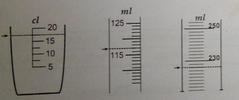
\includegraphics[scale=0.9]{images/td3img1.png}
\item Une éprouvette graduée contenant de l'eau, Akossi veut mesurer le volume d'un caillou.
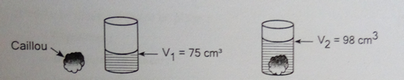
\includegraphics[scale=0.9]{images/td3img2.png}
\begin{enumerate}
\item Calcule le volume du caillou.
\item Akossi peut-il utiliser le procédé pour mesurer le volume d'un morceau de sucre? Donne ta raison.
\end{enumerate}
\end{enumerate}
\end{exo}

\begin{exo}
\begin{enumerate}
\item Recopie puis complète les phrases suivantes:
\begin{enumerate}
\item La solidification est le passage d'un corps de l'état \ldots \ldots à l'état solide.
\item La \ldots \ldots est le passage d'un corps de l'état liquide à l'état gazeux.
\item La fusion est le passage d'un corps de l'état solide à l'état \ldots \ldots.
\item La \ldots \ldots est le passage d'un corps de l'état gazeux à l'état liquide.
\item La sublimation est le passage d'un corps de l'état solide à l'état \ldots \ldots.
\end{enumerate}
\item Complète le texte suivant sans recopier:
Koffi sort du congélateur un morceau de glace et le dépose dans une casserole. L'eau est à l'état \ldots (a) \ldots . Quelques instants après, la glace fond. L'eau est passé de l'état \ldots (b) \ldots à l'état \ldots (c) \ldots . On parle de \ldots (d) \ldots de l'eau. Koffi se met à chauffer la casserole. Quelques instants plus tard il voit apparaître des bulles dans l'eau contenue dans la casserole. C'est le phénomène de l' \ldots (e) \ldots . Il baisse ensuite un peu la garde de son expérience et lorsqu'il revient, il n'y a plus d'eau dans la casserole. L'eau est passé de l'état \ldots (f) \ldots à l'état \ldots (g) \ldots. C'est la \ldots (h) \ldots.
\end{enumerate}
\end{exo}
\end{td}

\newpage
\begin{devoir}{COMPOSITION DU PREMIER TRIMESTRE}{\matiere}{\classe}{1}{1H 30}{16 décembre 2019}{\prof}
\begin{exo}[5]
Koffi a mesuré la masse d'une bougie et trouve $m=42,8g$. Il allume cette bougie qui s'éteint quelques instants après. Une deuxième pesée lui donne une nouvelle masse $m'=41,6g$.
\begin{enumerate}
\item \begin{enumerate}
\item Pourquoi la masse de la bougie a-t-elle diminuée?
\item De combien a-t-elle diminuée?
\end{enumerate}
\item La bougie allumée a été coiffée par un flacon contenant $1,5l$ d'air. Calcule la masse de bougie qui brûle dans $1l$ d'air.
\item Après la combustion, on verse un liquide limpide et incolore dans le flacon. Ce liquide devient blanc laiteux (on dit qu'il se trouble).
\begin{enumerate}
\item Quel est ce liquide?
\item Qu'est-ce que le trouble de ce liquide te dit?
\end{enumerate}
\end{enumerate}
\competence{•}{5}
\end{exo}

\begin{exo}[6]
\begin{enumerate}
\item Détermine le volume du liquide contenu dans chacun des récipients suivants:
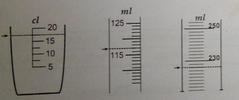
\includegraphics[scale=0.8]{images/td3img1.png}
\item Une éprouvette graduée contenant de l'eau, Akossi veut mesurer le volume d'un caillou.
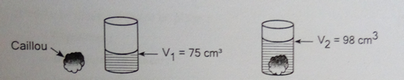
\includegraphics[scale=0.8]{images/td3img2.png}
\begin{enumerate}
\item Calcule le volume du caillou.
\item Akossi peut-il utiliser le procédé pour mesurer le volume d'un morceau de sucre? Donne ta raison.
\end{enumerate}
\end{enumerate}
\competence{•}{6}
\end{exo}

\begin{exo}[9]
\begin{enumerate}
\item Recopie puis complète les phrases suivantes:
\begin{enumerate}
\item La solidification est le passage d'un corps de l'état \ldots \ldots à l'état solide.
\item La \ldots \ldots est le passage d'un corps de l'état liquide à l'état gazeux.
\item La fusion est le passage d'un corps de l'état solide à l'état \ldots \ldots.
\item La \ldots \ldots est le passage d'un corps de l'état gazeux à l'état liquide.
\item La sublimation est le passage d'un corps de l'état solide à l'état \ldots \ldots.
\end{enumerate}
\item Complète le texte suivant sans recopier:
Koffi sort du congélateur un morceau de glace et le dépose dans une casserole. L'eau est à l'état \ldots (a) \ldots . Quelques instants après, la glace fond. L'eau est passé de l'état \ldots (b) \ldots à l'état \ldots (c) \ldots . On parle de \ldots (d) \ldots de l'eau. Koffi se met à chauffer la casserole. Quelques instants plus tard il voit apparaître des bulles dans l'eau contenue dans la casserole. C'est le phénomène de l' \ldots (e) \ldots . Il baisse ensuite un peu la garde de son expérience et lorsqu'il revient, il n'y a plus d'eau dans la casserole. L'eau est passé de l'état \ldots (f) \ldots à l'état \ldots (g) \ldots. C'est la \ldots (h) \ldots.
\end{enumerate}
\competence{•}{9}
\end{exo}
\tableofcompetences
\end{devoir}

\newpage
\begin{td}{\matiere}{\classe}{18 janvier 2020}{\prof}
\begin{exo}
Réponds par vrai ou faux aux affirmations suivantes:
\begin{enumerate}
\item Le volume d'un liquide est la place qu'il occupe dans le récipient.
\item La capacité d'un récipient est le volume de solide qu'il peut contenir lorsqu'il est plein.
\item La surface libre d'un liquide est la surface en contact avec l'air.
\item Les solides et les liquides ont une forme propre.
\item $250ml$=$0,00025m^3$
\item $2018cm^3$=$0,2018hl$
\end{enumerate}
\end{exo}
\end{td}

\begin{exo}
Ton professeur de Chimie met au tableau la formule chimique suivante: carbone + oxygène $\rightarrow$ dioxyde de carbone.
\begin{enumerate}
\item Quel nom donne-t-on à cette réaction?
\item Quels sont les réactifs de cette expérience?
\item Donne le nom du produit formé. Comment le met-on en évidence?
\item Quel est le réactif combustible?
\item Justifie que cette réaction est une transformation chimique.
\end{enumerate}
\end{exo}

\begin{exo}
On brûle 15g de soufre dans un bocal contenant de l'oxygène. Après quelques temps, il se forme un gaz.
\begin{enumerate}
\item De quel gaz s'agit-il?
\item Comment le met-on en évidence?
\item Cite quelques autres propriétés de ce gaz.
\item Après avoir définis les termes: réactifs et produits, cite les réactifs et le produit de cette expérience.
\item Sachant que 2g de soufre brûle dans 5g d'oxygène:
\begin{enumerate}
\item Quelle est la masse d'oxygène nécessaire à cette réaction?
\item Donne l'écriture chimique de cette réaction.
\item Est-il bon de respirer le gaz produit par cette réaction?
\end{enumerate}
\end{enumerate}
\end{exo}

\begin{exo}
Ouro, un élève de la classe de $6^{ème}$ est envoyé par ses parents pour acheter demi-kilogramme de viande. Arrivé, le boucher utilise un instrument comportant deux plateaux en métal. Dans l'un il met un gros clou et dans l'autre il met de la viande et lui dit que la viande fait demi-kilogramme.

\textbf{\underline{Consigne}}:
\begin{enumerate}
\item En quelle grandeur est exprimée la quantité de viande? Quelle est l'unité de mesure?
\item Quel est le nom de l'instrument de mesure?
\item Quels sont le nom et la nationalité de l'inventeur de cet instrument?
\item A travers un schéma, aide Ouro à comprendre le processus de mesure utilisé par le boucher.
\end{enumerate}
\end{exo}

\newpage
\begin{td}{\matiere}{\classe}{07 février 2020}{\prof}
\begin{exo}
\begin{enumerate}
\item Reproduis puis complète le tableau suivant:\\
\begin{tabular}{|l|p{4cm}|p{4cm}|p{4cm}|}
\hline 
Réaction chimique & Réactifs & Produit & Réactif pour identifier le produit formé \\ 
\hline 
Combustion du carbone &  &  &  \\ 
\hline 
Combustion du soufre &  &  & \\ 
\hline 
\end{tabular} 
\item Ecris la formule chimique des deux réactions chimiques de la question 1).
\end{enumerate}

\end{exo}

\begin{exo}
Complète la grille suivante:\\
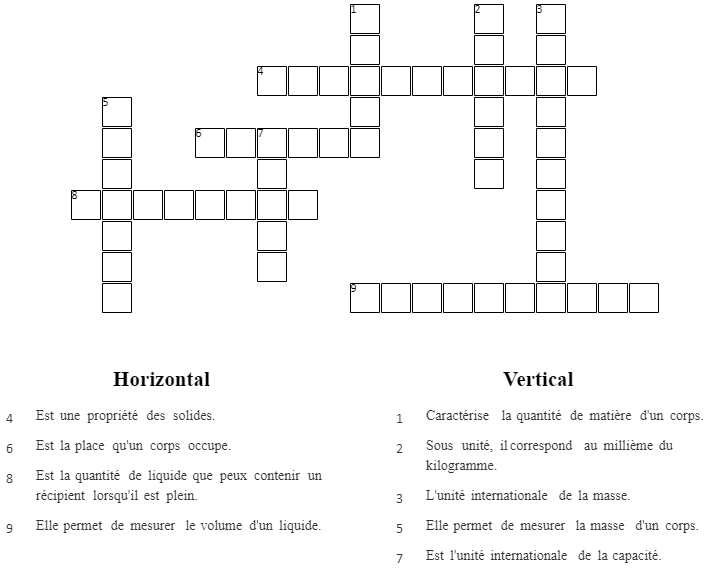
\includegraphics[scale=0.5]{images/mots_croises1.png}
\end{exo}

\begin{exo}
\begin{enumerate}
\item Décris la technique de la pesée simple.
\item Détermine la masse du solide S dans chacun des cas suivants:\\
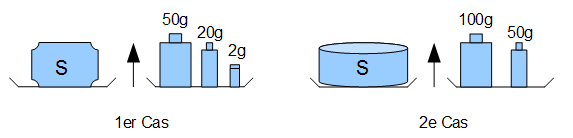
\includegraphics[scale=0.9]{images/masses_roberval1.png}
\item Convertis en gramme (g):
$10kg$ \qquad ; \qquad $0,2dag$ \qquad ; \qquad $10mg$ \qquad ; \qquad $250cg$.
\item Un camion pèse 1200 kilogrammes. Chargé, sa masse total est de 2,5 tonnes. Quelle est masses du chargement de ce camion?
\end{enumerate}

\end{exo}
\end{td}

\begin{devoir}{DEVOIR SURVEILLÉ DU DEUXIÈME TRIMESTRE}{\matiere}{\classe}{1}{1H 30}{13 février 2020}{\prof}
\begin{exo}[8]
Ouro, un élève de la classe de $6^{ème}$ est envoyé par ses parents pour acheter demi-kilogramme de viande. Arrivé, le boucher utilise un instrument comportant deux plateaux en métal. Dans l'un il met un gros clou et dans l'autre il met de la viande et lui dit que la viande fait demi kilogramme.

\textbf{\underline{Consigne}}:
\begin{enumerate}
\item En quelle grandeur est exprimée la quantité de viande? Quelle est l'unité de mesure?
\item Quel est le nom de l'instrument de mesure?
\item Avec un schéma à l'appui, aide Ouro à comprendre le processus de mesure utilisé par le boucher.
\end{enumerate}
\end{exo}

\vspace{0.5cm}
\begin{exo}[4,5]
\begin{multicols}{2}
Complète la grille ci-contre:\\
\textbf{Horizontal}\\
4- Est une propriété des solides.\\
6- Est la place qu'un corps occupe.\\
8- Est la quantité de matière que peut contenir un récipient lorsqu'il est plein.\\
9- Elle permet de mesurer le volume d'un liquide.\\


\textbf{Vertical}\\
1- Caractérise la quantité de matière d'un corps.\\
2- Sous unité, il correspond au millième du kilogramme.\\
3- L'unité internationale de la masse.\\
5- Elle permet de mesurer la masse d'un corps.\\
7- L'unité internationale de la capacité.\\
\vspace{1cm}
\begin{center}
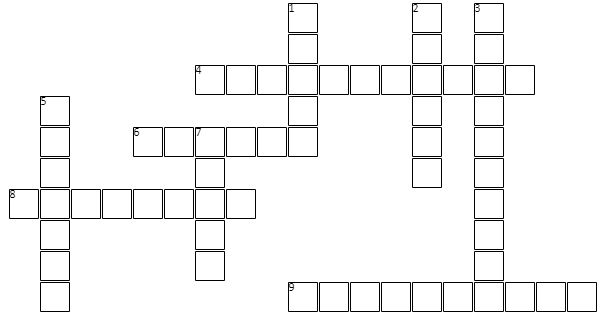
\includegraphics[scale=0.45]{images/dev2_2020_mots_croises.png}
\end{center}

\vspace{1cm}
\end{multicols}
\end{exo}

\vspace{0.5cm}
\begin{exo}[7,5]
\begin{enumerate}
\item Détermine la masse du solide S dans chacun des cas suivants:\\
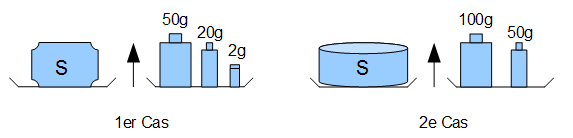
\includegraphics[scale=0.9]{images/masses_roberval1.png}
\item Convertis en gramme (g):
$10kg$ \qquad ; \qquad $0,2dag$ \qquad ; \qquad $10mg$ \qquad ; \qquad $250cg$.
\item Un professeur de PCT écrit au tableau la formule chimique suivante:\\ 
$Carbone \quad + \quad Oxygène \rightarrow Dioxyde \quad de \quad Carbone$.
\begin{enumerate}
\item Quel est le nom de la réaction traduite par cette formule?
\item Quels sont les réactifs de cette réaction chimique?
\item Quel est le produit.
\item Donne le nom du réactif qui permet d'identifier ce produit.
\item Quelle différence fais-tu entre une réaction chimique et une transformation physique?
\end{enumerate}
\end{enumerate}
\end{exo}

\end{devoir}

\begin{td}{\matiere}{\classe}{07 mars 2020}{\prof}
\begin{exo}
Du retour de l'école, tu surprends une dispute de tes parents au sujet de ton petit frère Komlavi qui est malade. Komlavi a de la fièvre et dit qu'il a froid. Cependant lorsqu'on votre maman le touche elle ressent beaucoup de chaleur. Votre maman dit: "Komlavi a de la température". Votre Papa estime que votre maman n'a pas raison car Komlavi dit qu'il a froid.\\

\textbf{\underline{Consigne:}}
\begin{enumerate}
\item Après avoir défini la température, dis si cette phrase: \emph{"Komlavi a de la température"} prononcée par votre maman est correcte. Sinon corrige-la.
\item Vos parents n'arrivent pas à se mettre d'accord sur la température du corps de votre frère, comment peux-tu les aider?
\end{enumerate}
\end{exo}

\vspace{0.2cm}

\begin{exo}
\setlength{\columnseprule}{1pt}
\begin{multicols}{2}
\begin{enumerate}
\item Réponds par vrai ou faux et corrige les affirmations fausses:
\begin{enumerate}
\item L'instrument de mesure de la température est la balance.
\item Le degrés celsius est une unité de la masse.
\item Le thermomètre médical permet de déterminer la température d'un appartement.
\item Lorsqu'un corps reçoit de la chaleur sa température augmente.
\end{enumerate}
\item Quelles est la température indiquées dans chacun des cas suivants?\\
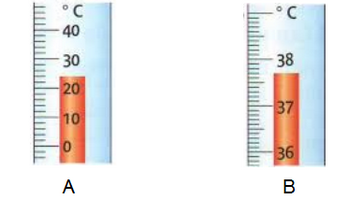
\includegraphics[scale=0.8]{images/td_07_03_2020_temperature.png}
\end{enumerate}
\end{multicols}
\end{exo}

\vspace{0.2cm}

\begin{exo}
Ariane a pesé un objet et a trouvé $450g$.
\begin{enumerate}
\item Que représente $450g$ pour cet objet?
\competence{reconnaître une masse à l'aide de l'unité}{1}
\item Définir cette grandeur.
\competence{définir la masse}{1}
\item Quel instrument de mesure a- t- elle utilisé?
\competence{connaître l'instrument de mesure de la masse}{1}
\item Quelles sont les masses marquées possibles qu'elle aurait utilisées?
\competence{manipuler les masses marquées}{1}
\end{enumerate}
\end{exo}

\vspace{0.2cm}

\begin{exo}
On brûle le soufre dans $1l$ d'air.
\begin{enumerate}
\item Donne le nom du produit obtenu.
\item Comment peut- on reconnaître ce gaz?
\competence{nommer et identifier le produit formé au cours de la combustion du soufre}{2}
\item Calcule le volume d'oxygène contenu dans le flacon.
\competence{utiliser la composition en volume de l'air}{1}
\item La masse du soufre augmente ou diminue- t- elle dans le flacon? Pourquoi?
\competence{lois d'un réaction chimique}{1}
\item Écris la formule chimique de cette réaction.
\competence{écrire la formule chimique de la combustion du soufre}{1}
\item Avant la combustion la masse du soufre est de $32,6g$. Après le combustion, sa masse est $32,2g$. Calcule la masse du soufre disparue.
\competence{calcule la masse consommée d'un réactif}{1}
\item Calcule la masse du soufre qui peut brûler dans $10l$ d'air.
\competence{utiliser la proportionnalité pour calculer une masse}{1}
\end{enumerate}
\end{exo}
\end{td}

\begin{devoir}{COMPOSITION DU DEUXIÈME TRIMESTRE}{\matiere}{\classe}{1}{1H 30}{28 mai 2019}{\prof}
\begin{exo}[6]
Au retour de l'école, tu surprends une dispute de tes parents au sujet de ton petit frère Komlavi qui est malade. Komlavi a de la fièvre et dit qu'il a froid. Cependant lorsqu'on votre maman le touche elle ressent beaucoup de chaleur. Votre maman dit: "Komlavi a de la température". Votre Papa estime que votre maman n'a pas raison car Komlavi dit qu'il a froid.\\

\textbf{\underline{Consigne:}}
\begin{enumerate}
\item Après avoir défini la température, dis si cette phrase: \emph{"Komlavi a de la température"} prononcée par votre maman est correcte. Sinon corrige-la.
\item Vos parents n'arrivent pas à se mettre d'accord sur la température du corps de votre frère, comment peux-tu les aider?
\item Quels sont les effets que la chaleur peut avoir sur un corps?
\end{enumerate}
\end{exo}

\vspace{0.2cm}

\begin{exo}[4]
\setlength{\columnseprule}{1pt}
\begin{multicols}{2}
\begin{enumerate}
\item Réponds par vrai ou faux:
\begin{enumerate}
\item Le degrés celsius est une unité de la température.
\item L'instrument de mesure de la masse est le thermomètre.
\item Lorsqu'un corps reçoit de la chaleur sa température diminue.
\item La valeur 450$cm^3$ désigne la masse d'un corps.\\
\end{enumerate}
\item Quelles est la température indiquées dans chacun des cas suivants?\\
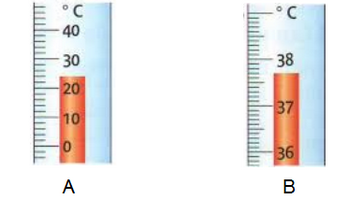
\includegraphics[scale=0.8]{images/td_07_03_2020_temperature.png}
\end{enumerate}
\end{multicols}
\end{exo}

\vspace{0.2cm}

\begin{exo}[4]
Stéphanie a pesé un objet et a trouvé $450g$.
\begin{enumerate}
\item Que représente $450g$ pour cet objet?
\competence{reconnaître une masse à l'aide de l'unité}{1}
\item Définis cette grandeur et donne le nom de l'instrument qui permet de la mesurer?
\item Quelles sont les masses marquées possibles qu'elle aurait utilisées?
\item Sachant que le volume de ce corps est $750cm^3$, calcule sa masse volumique.
\end{enumerate}
\end{exo}

\vspace{0.2cm}

\begin{exo}[6]
On brûle le soufre dans $1l$ d'air.
\begin{enumerate}
\item Donne le nom du produit obtenu.
\item Comment peut- on reconnaître ce gaz?
\competence{nommer et identifier le produit formé au cours de la combustion du soufre}{2}
\item Calcule le volume d'oxygène contenu dans le flacon.
\competence{utiliser la composition en volume de l'air}{1}
\item La masse du soufre augmente ou diminue- t- elle dans le flacon? Pourquoi?
\competence{lois d'un réaction chimique}{1}
\item Écris la formule chimique de cette réaction.
\competence{écrire la formule chimique de la combustion du soufre}{1}
\item Avant la combustion la masse du soufre est de $32,6g$. Après le combustion, sa masse est $32,2g$. Calcule la masse du soufre disparue.
\competence{calcule la masse consommée d'un réactif}{1}
\item Calcule la masse du soufre qui peut brûler dans $10l$ d'air.
\competence{utiliser la proportionnalité pour calculer une masse}{1}
\end{enumerate}
\end{exo}
\end{devoir}

\end{document}
